\documentclass[12pt,a4paper]{article}

% Page layout
\usepackage{geometry}
\geometry{margin=2.5cm}

% Turkish (XeLaTeX)
\usepackage{fontspec}
\usepackage{polyglossia}
\setdefaultlanguage{turkish}
\setmainfont{Latin Modern Roman}

% Math, tables, figures
\usepackage{amsmath}
\usepackage{siunitx}
\usepackage{booktabs}
\usepackage{graphicx}
\usepackage{float}
\usepackage{caption}
\usepackage{subcaption}

% Typography and links
\usepackage{microtype}
\usepackage{hyperref}
\hypersetup{
  colorlinks=true,
  linkcolor=black,
  citecolor=black,
  urlcolor=black
}

% Bibliography (IEEE style)
\usepackage[backend=biber,style=ieee]{biblatex}
\addbibresource{refs.bib}

% Title
\title{Göz Retinası Görüntülerinde Damar Yapısı Belirginleştirme ve Analizi}
\author{Recep Öztürk \\ YMH423 Görüntü İşleme Teknikleri}
\date{\today}

\begin{document}
\maketitle

% Abstract + Keywords (contains abstract environment)
\begin{abstract}
Bu çalışmada, fundus retina görüntülerinde damar yapısının otomatik olarak segmentasyonu ve segmentasyon çıktısından morfolojik göstergelerin çıkarımı sunulmuştur. Deneyler, piksel düzeyinde damar anotasyonları içeren FIVES veri seti üzerinde gerçekleştirilmiştir \cite{jin2022fives}. Ön işleme aşamasında retina görüş alanı (FOV) maskeleme işlemi Otsu eşikleme ve morfolojik işlemler ile elde edilmiş; görüntüler retina merkezli olacak şekilde kırpılıp $512\times512$ çözünürlüğe yeniden ölçeklenmiştir. Segmentasyon için U-Net mimarisi kullanılmış \cite{ronneberger2015unet}; eğitim sırasında ikili çapraz-entropy (BCE) ve Dice kaybının birleşimi tercih edilmiştir. Veri artırma adımları Albumentations kütüphanesi ile uygulanmıştır \cite{buslaev2020albumentations}.

Test kümesinde (200 görüntü) elde edilen ortalama performans; Dice $0.8059\pm0.0752$, IoU $0.6807\pm0.0946$, kesinlik (precision) $0.8100\pm0.0760$ ve duyarlılık (recall) $0.8083\pm0.0883$ olarak ölçülmüştür. Segmentasyon çıktıları üzerinden damar yoğunluğu, iskelet uzunluğu ve dallanma sayısı hesaplanmış; damar yoğunluğu ortalamada korunurken, iskelet uzunluğu ve dallanma sayısında azalma eğilimi gözlenmiştir. Sonuçlar, derin öğrenme tabanlı damar segmentasyonunun morfolojik damar analizi için uygulanabilir bir temel oluşturduğunu göstermektedir.
\end{abstract}

\vspace{0.5em}
\noindent\textbf{Anahtar Kelimeler:} retina, fundus, damar segmentasyonu, U-Net, FOV maskeleme, Dice, morfolojik analiz


% Main sections
\section{Giriş}
Retina damar ağı, fundus görüntüleri üzerinden doğrudan gözlemlenebilen ve hem oftalmolojik hem de sistemik durumlarla ilişkili olabilen önemli bir biyobelirteçtir. Bu nedenle retina damarlarının güvenilir biçimde ayrıştırılması (segmentasyonu), damar morfometrilerinin nesnel olarak ölçülmesi ve klinik karar destek süreçlerine veri üretimi açısından kritik bir ön adımdır \cite{jin2022fives}. Bununla birlikte damar segmentasyonu; düşük kontrast, ince damar uçları, görüntü aydınlatma farklılıkları ve patolojik yapıların damar benzeri görünmesi gibi nedenlerle zorlu bir bilgisayarlı görü problemidir.

Bu çalışma, fundus retina görüntülerinde damar yapısının derin öğrenme tabanlı segmentasyonunu ve segmentasyon çıktısından temel damar morfolojik göstergelerinin otomatik çıkarımını hedeflemektedir. Çalışmada FIVES veri seti kullanılmıştır \cite{jin2022fives}. Segmentasyon modeli olarak biyomedikal görüntü segmentasyonunda yaygın kullanılan U-Net mimarisi tercih edilmiştir \cite{ronneberger2015unet}. Eğitimde genellemeyi artırmak amacıyla veri artırma adımları Albumentations ile uygulanmıştır \cite{buslaev2020albumentations}. Ayrıca, metrik hesaplarının retina dışı alanlardan etkilenmesini azaltmak için görüş alanı (FOV) maskeleme temelli bir ön işleme hattı kurulmuştur.

Bu raporun katkıları aşağıdaki şekilde özetlenebilir:
\begin{itemize}
    \item FOV maskeleme ve retina merkezli kırpma ile veri geometrisinin standardize edilmesi ve değerlendirme metriklerinin daha anlamlı hâle getirilmesi,
    \item U-Net tabanlı model ile damar segmentasyonu için uçtan uca bir eğitim ve test sürecinin kurulması,
    \item Segmentasyon maskeleri üzerinden damar yoğunluğu, iskelet uzunluğu ve dallanma sayısı gibi göstergelerin hesaplanarak morfolojik analiz katmanının eklenmesi.
\end{itemize}

Raporun geri kalanı şu şekilde düzenlenmiştir: Bölüm~2'de arka plan ve ilgili çalışmalar özetlenmekte; Bölüm~3'te kullanılan yöntem, ön işleme adımları, model mimarisi ve değerlendirme metrikleri ayrıntılandırılmaktadır. Bölüm~4 deneysel kurulum ve eğitim ayarlarını sunmakta; Bölüm~5 nicel ve nitel sonuçları, ayrıca damar analizi bulgularını raporlamaktadır. Bölüm~6'da bulgular tartışılmakta ve sınırlılıklar değerlendirilmektedir. Son olarak Bölüm~7'de sonuçlar ve gelecekte yapılabilecek iyileştirmeler verilmektedir.

\section{Arka Plan ve İlgili Çalışmalar}
\subsection{Retina Damar Segmentasyonu}
Retina damar segmentasyonu, görüntüdeki damar piksellerinin arka plandan ayrıştırılması problemidir. İnce damarların düşük kontrastla görünmesi, aydınlatma farklılıkları ve optik disk gibi anatomik yapıların damar benzeri kenarlar üretmesi, hata olasılığını artırır. Segmentasyon başarımı genellikle Dice ve IoU gibi örtüşme temelli metriklerle raporlanır. Bununla birlikte, yüksek Dice değerleri her zaman damar topolojisinin (ince uçlar, dallanmalar) doğru yakalandığı anlamına gelmeyebilir; bu nedenle morfolojik/iskelet tabanlı analizler ek bir değerlendirme katmanı sağlar.

\subsection{FIVES Veri Seti}
Bu çalışmada FIVES veri seti kullanılmıştır \cite{jin2022fives}. FIVES, fundus görüntülerinde damar yapıları için piksel düzeyinde anotasyonlar sunar ve derin öğrenme tabanlı damar segmentasyonu çalışmalarında yaygın olarak kullanılan güncel veri setlerinden biridir. Bu raporda veri seti eğitim/test ayrımıyla kullanılmış; ayrıca eğitim verisi içerisinden doğrulama (validation) alt kümesi ayrılarak hiperparametre ve checkpoint seçimi yapılmıştır.

\subsection{U-Net ve Biyomedikal Segmentasyon}
U-Net mimarisi, encoder--decoder yapısı ve skip connection'lar sayesinde hem bağlamsal bilgiyi hem de yerel detayları koruyarak segmentasyon çıktısı üretir \cite{ronneberger2015unet}. Özellikle biyomedikal görüntülerde sınırlı veri koşullarında başarılı olması, mimarinin bu problem için güçlü bir temel (baseline) olmasını sağlamaktadır.

\subsection{Veri Artırma}
Derin öğrenme modellerinde genellemeyi artırmak için veri artırma (augmentation) yaygın bir yaklaşımdır. Bu çalışmada dönüşüm işlemleri Albumentations kütüphanesi ile uygulanmıştır \cite{buslaev2020albumentations}. Augmentation adımları, eğitim sırasında görüntü ve maske üzerinde eş zamanlı uygulanarak geometrik uyum korunmuştur.

\section{Materyal ve Yöntem}
Bu bölümde veri hazırlama, ön işleme, model mimarisi, kayıp fonksiyonu ve değerlendirme ölçütleri sunulmaktadır.

\subsection{Veri Seti ve Bölme}
FIVES veri seti eğitim ve test olacak şekilde ayrılmıştır \cite{jin2022fives}. Eğitim kümesi içerisinden sabit bir rastgelelik tohumu (seed) kullanılarak doğrulama alt kümesi ayrılmıştır. Bu yaklaşım, model seçimi ve aşırı uyumun (overfitting) izlenmesi için gereklidir.

\subsection{Ön İşleme: FOV Maskeleme, Kırpma ve Yeniden Ölçekleme}
Fundus görüntülerinde retina dışında kalan siyah alanlar (background) hem eğitim sinyalini hem de metrikleri olumsuz etkileyebilir. Bu nedenle görüş alanı (FOV) maskesi üretilmiştir. FOV üretim hattı özetle şu adımlardan oluşur:
\begin{enumerate}
    \item RGB görüntünün yeşil kanalının çıkarılması ve Gauss bulanıklaştırma,
    \item Otsu yöntemi ile otomatik eşikleme,
    \item Morfolojik kapama/açma işlemleri ile maske temizleme,
    \item En büyük bağlı bileşenin seçilmesi ile retina bölgesinin izole edilmesi.
\end{enumerate}
Elde edilen FOV maskesi kullanılarak retina merkezli kare kırpma (crop) uygulanmış ve görüntüler $512\times512$ çözünürlüğe yeniden ölçeklenmiştir. Aynı geometrik dönüşümler görüntü, damar yer gerçeği (GT) maskesi ve FOV maskesi üzerinde tutarlı biçimde uygulanmıştır.

\subsection{Veri Artırma}
Eğitim sırasında genellemeyi artırmak için aşağıdaki dönüşümler kullanılmıştır \cite{buslaev2020albumentations}:
\begin{itemize}
    \item Yatay çevirme (HorizontalFlip, $p=0.5$),
    \item Dikey çevirme (VerticalFlip, $p=0.2$),
    \item Döndürme (Rotate, limit $\pm 15^\circ$, $p=0.5$),
    \item Parlaklık/kontrast değişimi (RandomBrightnessContrast, limit $\pm 0.15$, $p=0.5$).
\end{itemize}
Doğrulama ve test aşamalarında augmentasyon uygulanmamıştır.

\subsection{Model Mimarisi: U-Net}
Segmentasyon modeli olarak U-Net kullanılmıştır \cite{ronneberger2015unet}. Mimari, downsampling (encoder) ve upsampling (decoder) bloklarından oluşur. Encoder aşamasında özellik haritaları (feature maps) daha soyut temsillere dönüştürülürken, decoder aşamasında uzamsal çözünürlük geri kazanılır. Skip connection'lar, encoder'daki yüksek çözünürlüklü detayların decoder'a aktarılmasını sağlayarak ince damarların yakalanmasını destekler.

\subsection{Kayıp Fonksiyonu}
Model, ham logit çıktıları üretir. Eğitimde piksel bazlı ikili sınıflandırma için \texttt{BCEWith\-Logits\-Loss} ve örtüşme kalitesini doğrudan optimize eden Dice kaybı birleştirilmiştir:
\begin{equation}
\mathcal{L} = \lambda \, \mathcal{L}_{BCE} + (1-\lambda)\, \mathcal{L}_{Dice},
\end{equation}
burada $\lambda=0.5$ seçilmiştir. Bu kombinasyon, sınıf dengesizliği ve ince damarların kaçırılması (FN) gibi durumlarda daha kararlı öğrenme sağlamayı amaçlar.

\subsection{Değerlendirme Metrikleri}
Model başarımı Dice, IoU, precision ve recall metrikleri ile raporlanmıştır. Test aşamasında logit çıktıları sigmoid fonksiyonu ile olasılığa dönüştürülmüş ve $0.5$ eşik değeri ile ikili maske elde edilmiştir. Metriklerin daha anlamlı olması için, mümkün olan durumlarda ölçümler FOV bölgesi odaklı değerlendirilmiştir.

\subsection{Segmentasyon Sonrası Damar Analizi}
Segmentasyon maskeleri üzerinden üç temel gösterge hesaplanmıştır:
\begin{itemize}
    \item \textbf{Damar yoğunluğu (vessel density):} damar piksel oranı,
    \item \textbf{İskelet uzunluğu (skeleton length):} iskeletleştirilmiş damar piksellerinin sayısı,
    \item \textbf{Dallanma sayısı (branch count):} iskelet üzerinde dallanma noktalarının sayısı.
\end{itemize}
Bu göstergeler, segmentasyon metriklerinin ötesinde damar topolojisinin ve ince yapıların korunup korunmadığına dair ek bilgi sağlar.

\section{Deneysel Kurulum}
\subsection{Çalışma Ortamı}
Deneyler Google Colab ortamında GPU hızlandırma kullanılarak yürütülmüştür. Uygulama PyTorch tabanlı olarak gerçekleştirilmiş; veri artırma için Albumentations kullanılmıştır \cite{buslaev2020albumentations}.

\subsection{Eğitim Ayarları}
Model eğitiminde aşağıdaki hiperparametreler kullanılmıştır:
\begin{itemize}
    \item Görüntü boyutu: $512\times512$,
    \item Batch boyutu: 4,
    \item Epoch sayısı: 15,
    \item Optimizasyon: Adam,
    \item Öğrenme oranı: $1\times10^{-3}$,
    \item Rastgelelik tohumu (seed): 42.
\end{itemize}

\begin{table}[H]
\centering
\caption{Eğitim hiperparametreleri.}
\label{tab:hyperparams}
\begin{tabular}{ll}
\toprule
\textbf{Parametre} & \textbf{Değer} \\
\midrule
Girdi çözünürlüğü & $512\times512$ \\
Batch boyutu & 4 \\
Epoch sayısı & 15 \\
Optimizasyon & Adam \\
Öğrenme oranı & $1\times10^{-3}$ \\
Seed & 42 \\
\bottomrule
\end{tabular}
\end{table}

\subsection{Model Seçimi ve Checkpoint}
Eğitim sürecinde doğrulama kümesi metrikleri izlenmiş ve en iyi doğrulama performansını veren model checkpoint olarak kaydedilmiştir. Test sonuçları, bu en iyi model üzerinden raporlanmıştır.

\section{Sonuçlar}
Bu bölümde eğitim dinamikleri, nicel test sonuçları, nitel örnekler ve damar analizi bulguları sunulmaktadır.

\subsection{Eğitim ve Doğrulama Eğrileri}
Şekil~\ref{fig:trainloss} eğitim kaybı (loss) değişimini, Şekil~\ref{fig:valmetrics} doğrulama metriklerinin epoch'lara göre değişimini göstermektedir.

\begin{figure}[H]
\centering
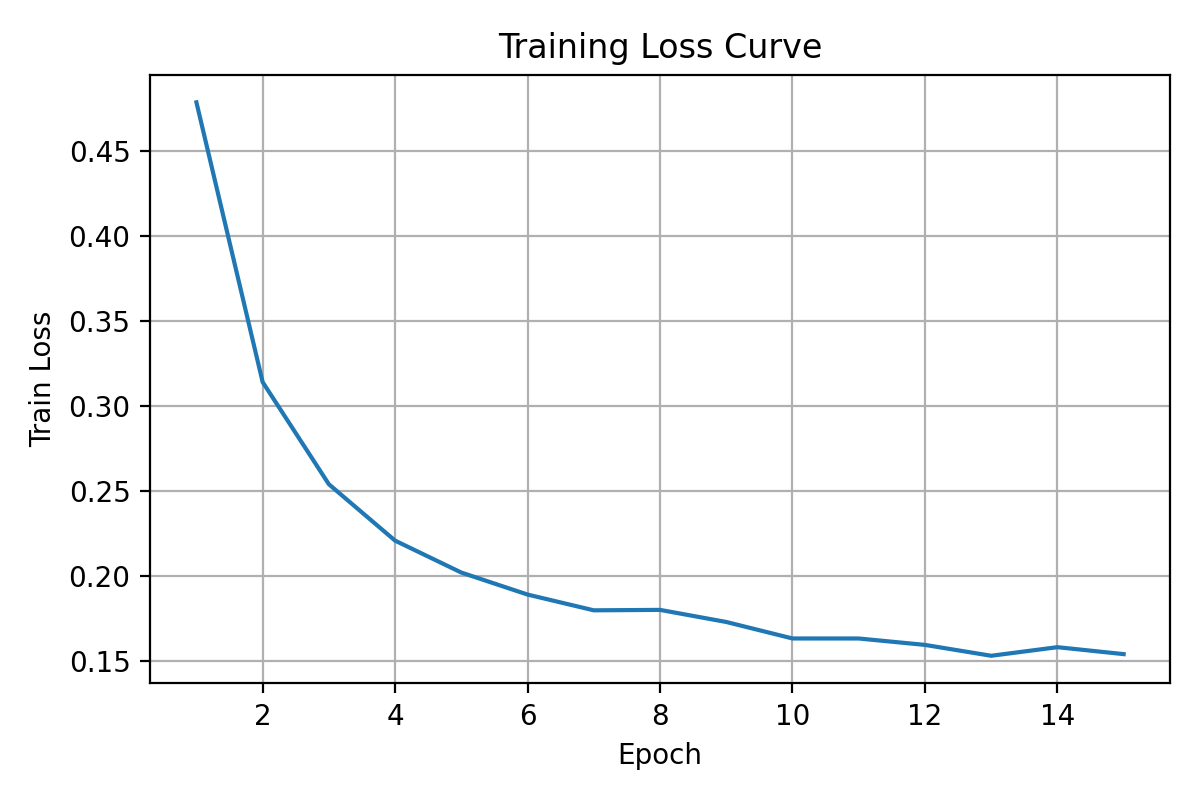
\includegraphics[width=0.85\linewidth]{figures/train_loss_curve.png}
\caption{Eğitim kaybının epoch'lara göre değişimi.}
\label{fig:trainloss}
\end{figure}

\begin{figure}[H]
\centering
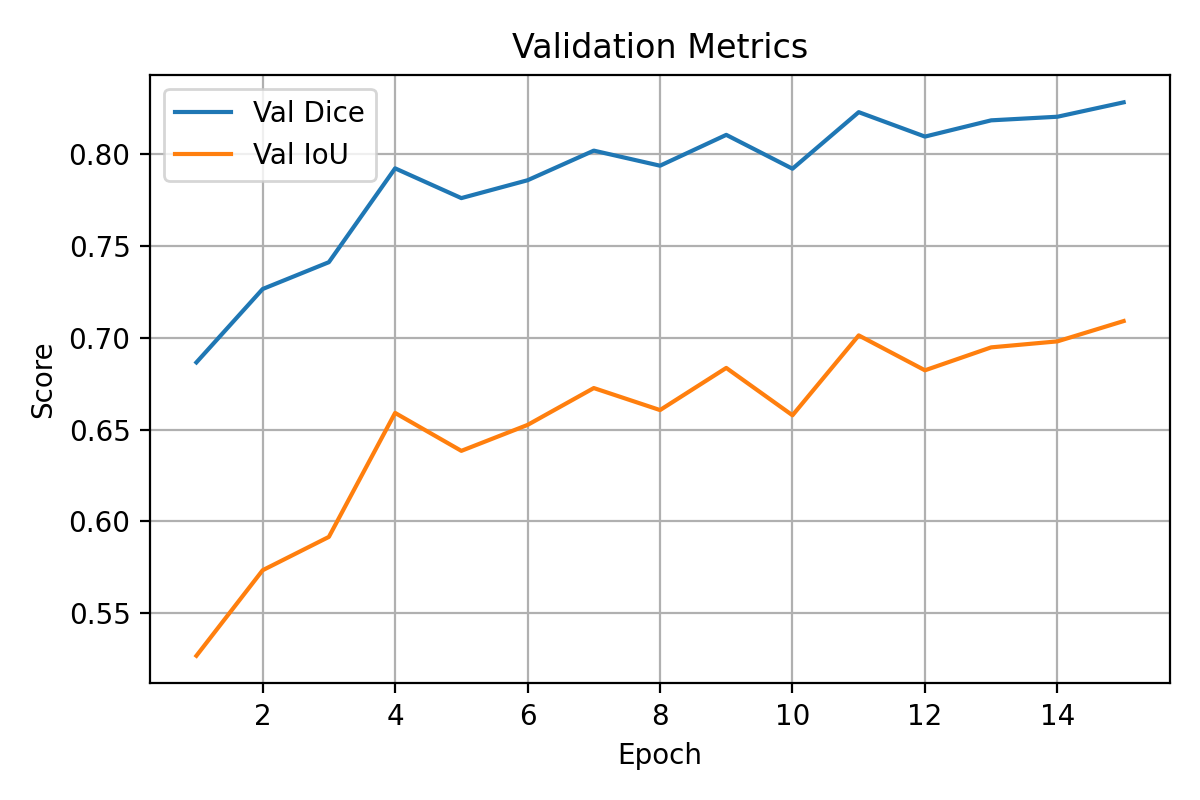
\includegraphics[width=0.85\linewidth]{figures/val_metrics_curve.png}
\caption{Doğrulama metriklerinin epoch'lara göre değişimi.}
\label{fig:valmetrics}
\end{figure}

\subsection{Nicel Test Performansı}
Test kümesinde (200 görüntü) görüntü başına ortalama (macro) metrikler Tablo~\ref{tab:test_macro}'te verilmiştir. Buna ek olarak, tüm test pikselleri üzerinde TP/FP/FN toplamları üzerinden hesaplanan piksel-ağırlıklı (micro) metrikler Tablo~\ref{tab:test_micro}'te sunulmuştur.

\begin{table}[H]
\centering
\small
\caption{Test kümesi macro metrikleri (mean$\pm$std).}
\label{tab:test_macro}
\begin{tabular}{lcc}
\toprule
\textbf{Metrik} & \textbf{Ortalama} & \textbf{Std. Sapma} \\
\midrule
Dice & 0.805876 & 0.075225 \\
IoU  & 0.680749 & 0.094570 \\
Precision & 0.809995 & 0.075987 \\
Recall & 0.808258 & 0.088333 \\
\bottomrule
\end{tabular}
\end{table}

\begin{table}[H]
\centering
\small
\caption{Test kümesi micro metrikleri (global TP/FP/FN üzerinden).}
\label{tab:test_micro}
\begin{tabular}{lc}
\toprule
\textbf{Metrik} & \textbf{Değer} \\
\midrule
Dice & 0.820165 \\
IoU  & 0.695152 \\
Precision & 0.816622 \\
Recall & 0.823739 \\
\bottomrule
\end{tabular}
\end{table}

\subsection{Nitel Sonuçlar}
Şekil~\ref{fig:qualitative} seçili örneklerde gerçek maske (GT), model tahmini ve hata karakterini (FP/FN) görsel olarak sunar. İyi performans gösteren örneklerin yanı sıra, ince damar uçlarında kaçırmaların (FN) belirginleştiği zor örnekler de raporlanmıştır.

\begin{figure}[H]
\centering
\small
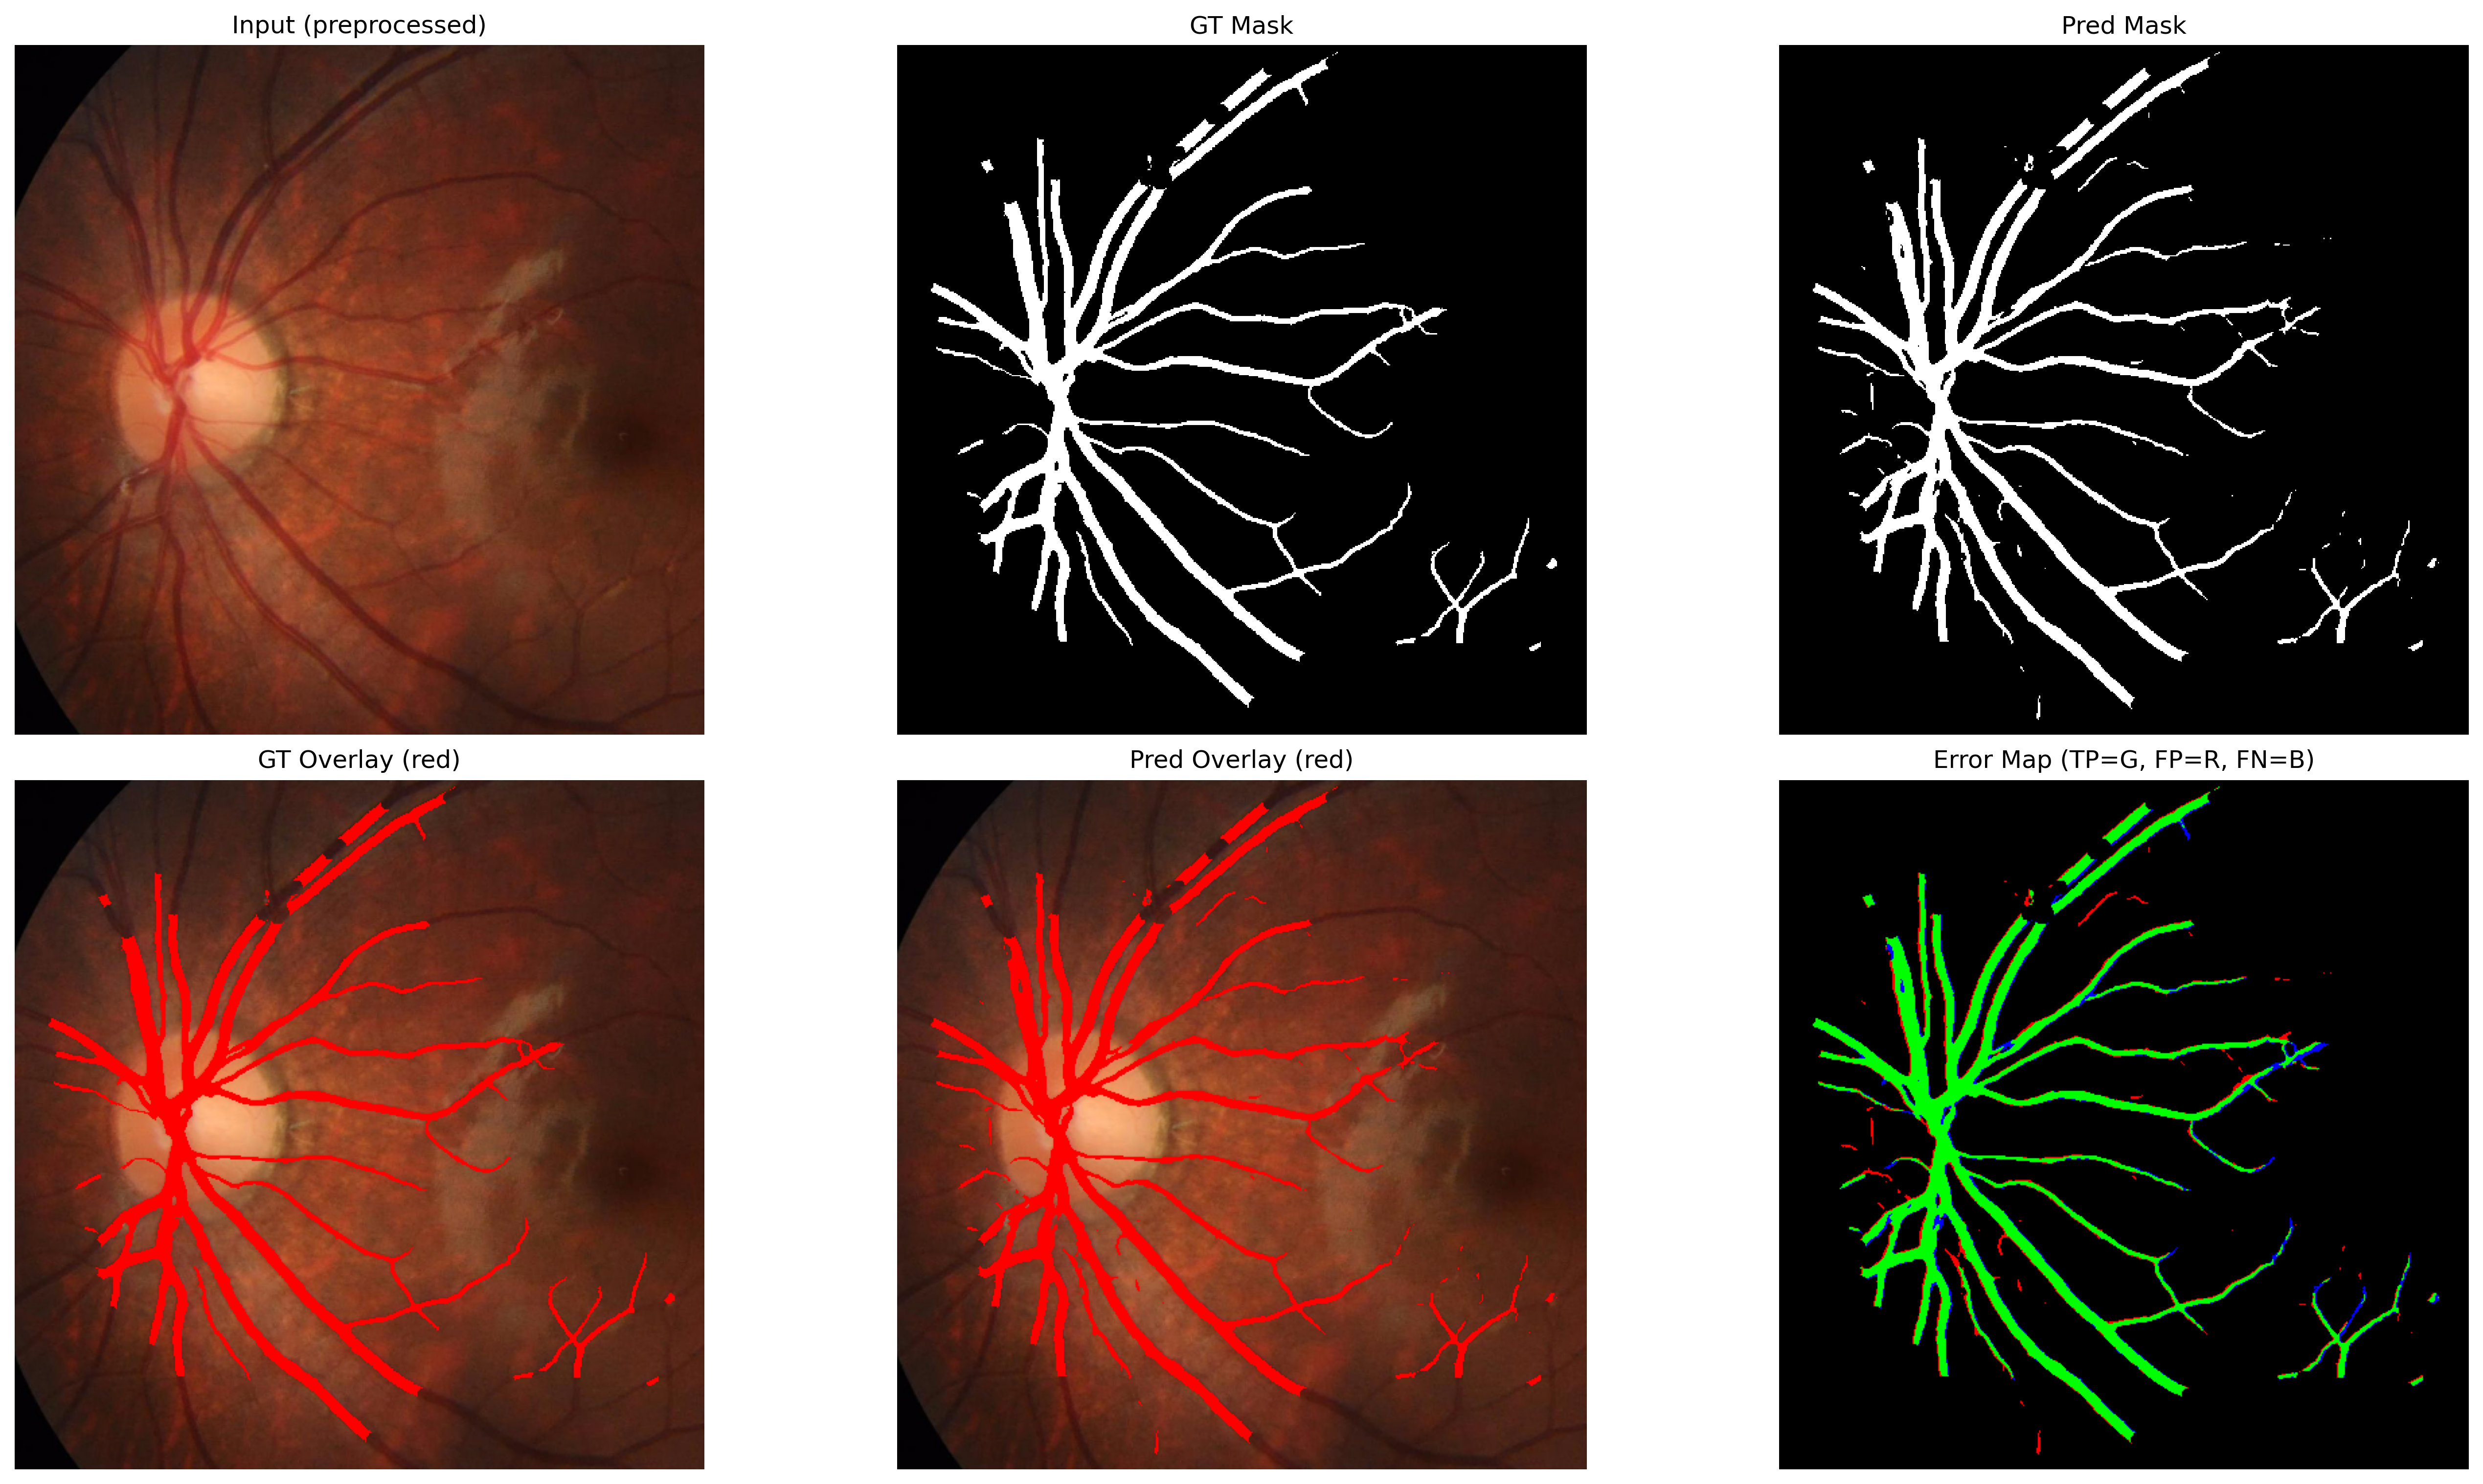
\includegraphics[width=0.48\linewidth]{figures/test_vis_160_N.png}\hfill
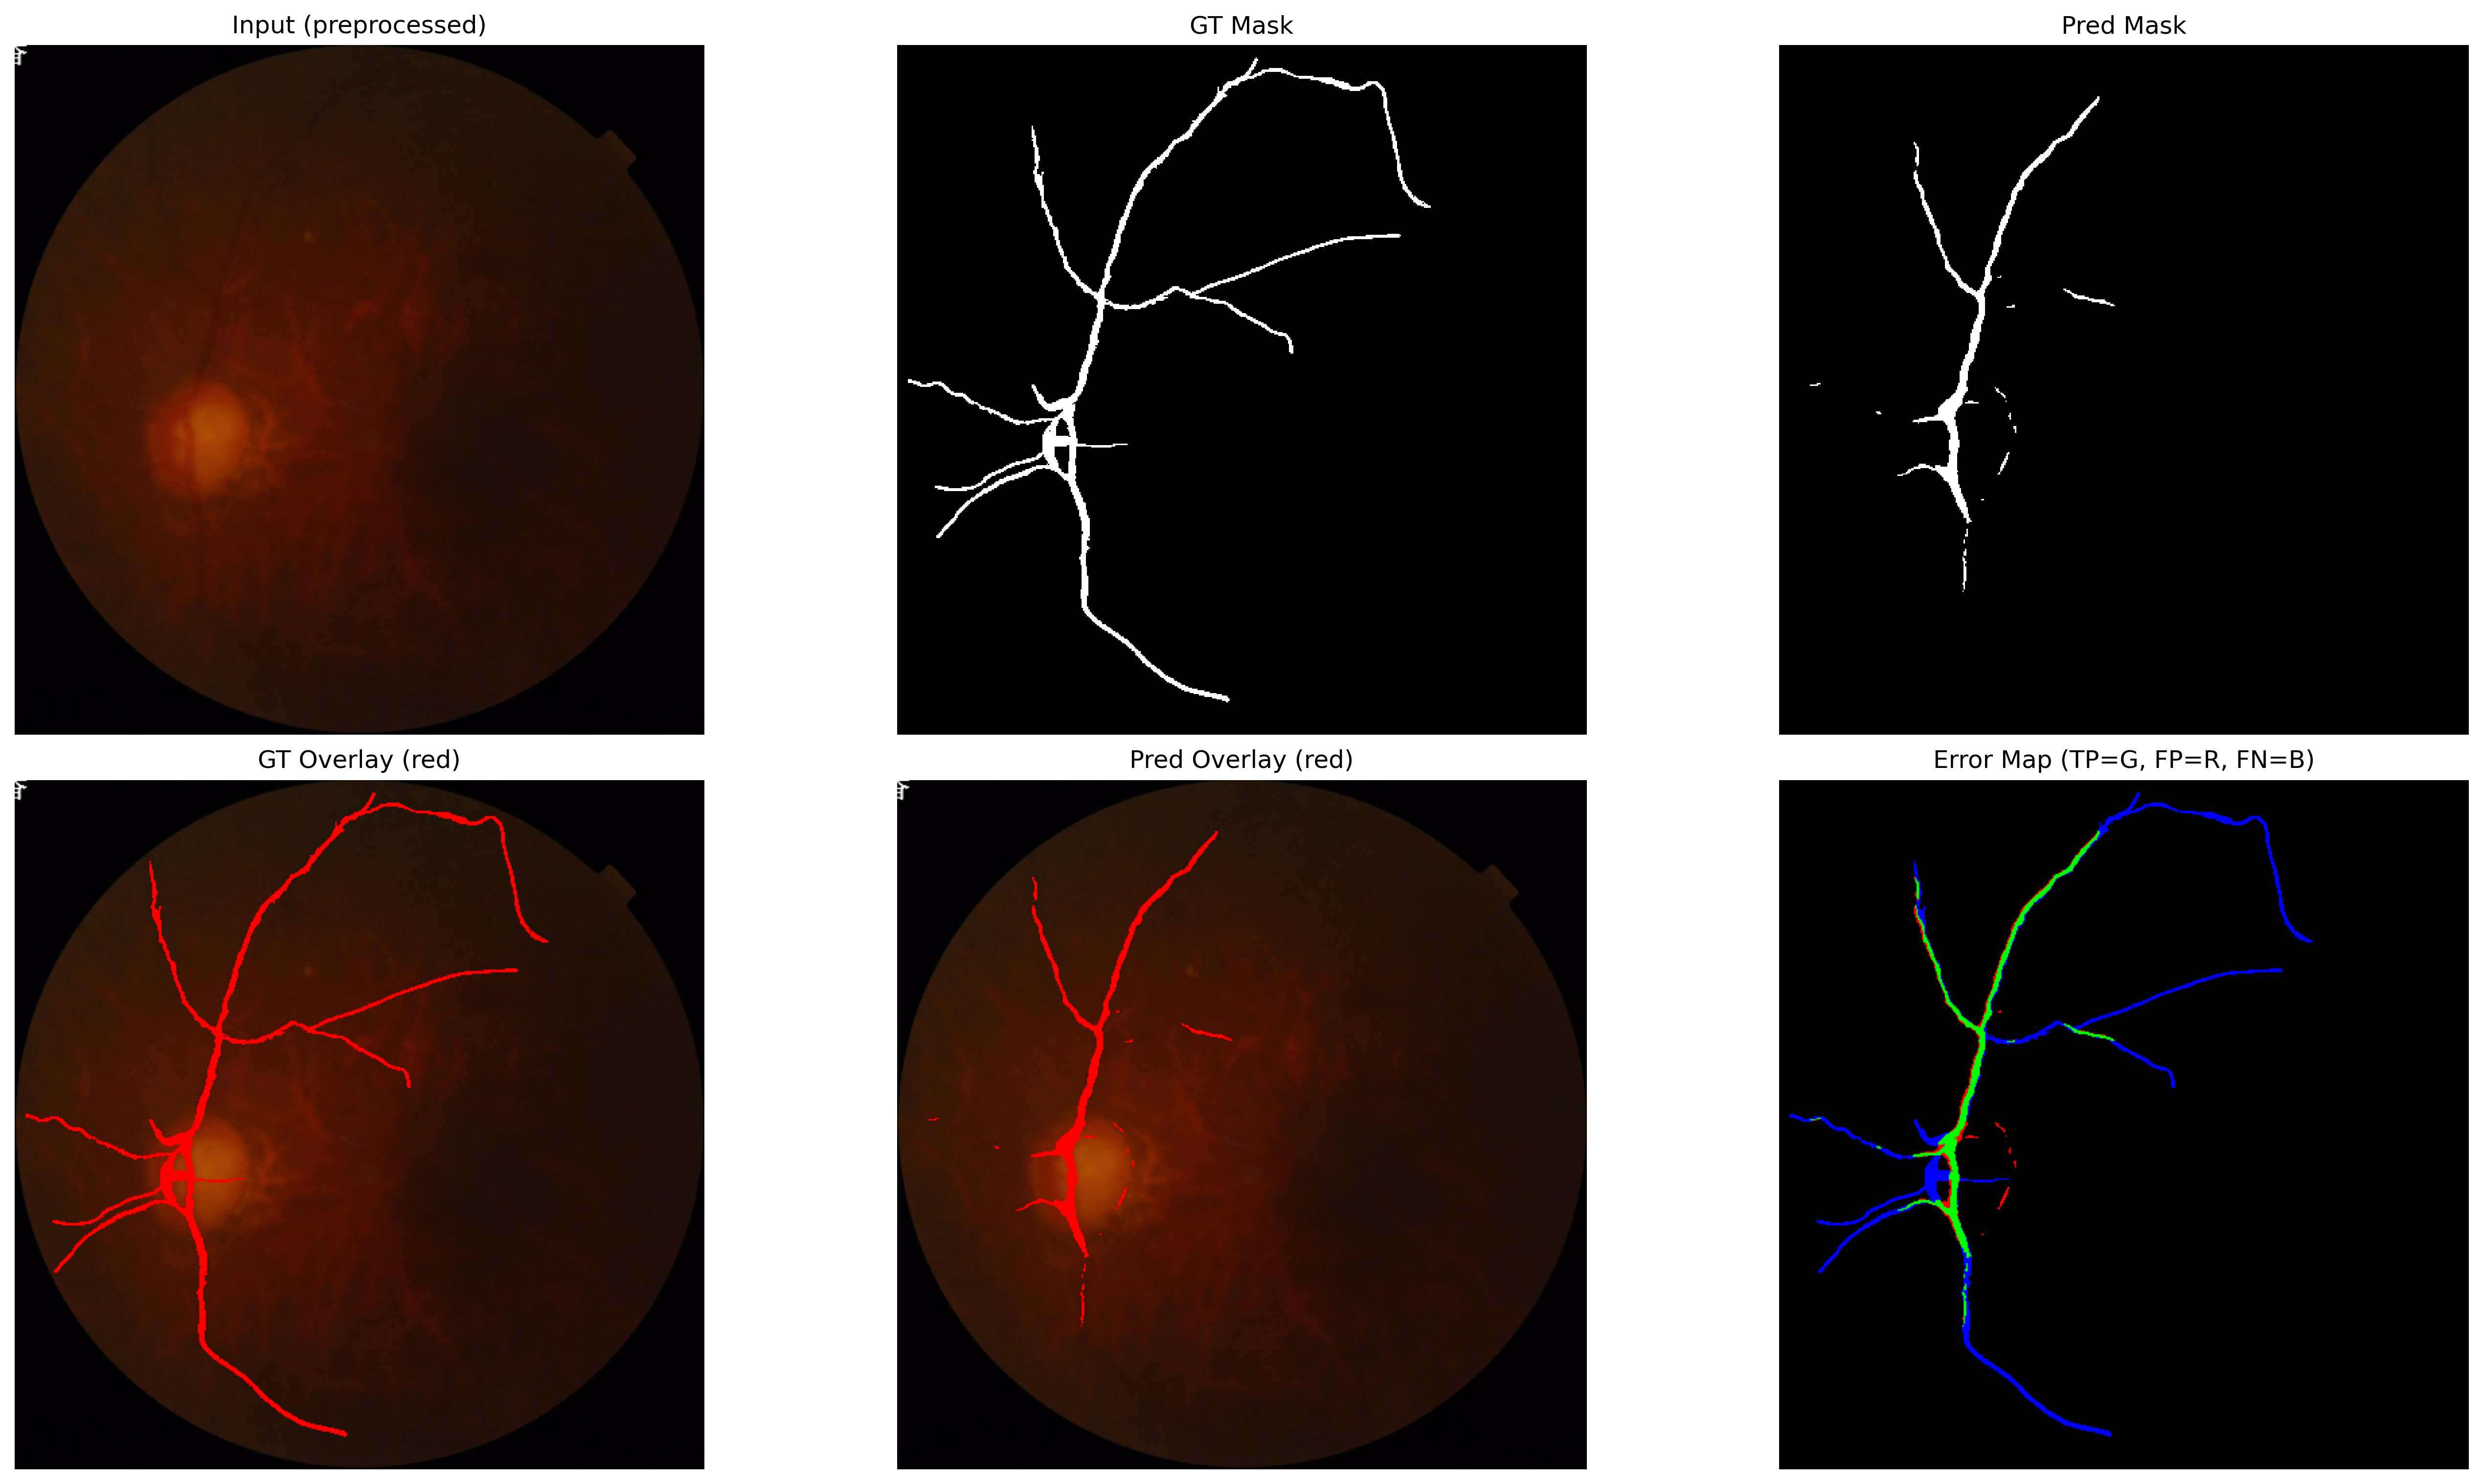
\includegraphics[width=0.48\linewidth]{figures/test_vis_136_G.png}\\
\vspace{0.5em}
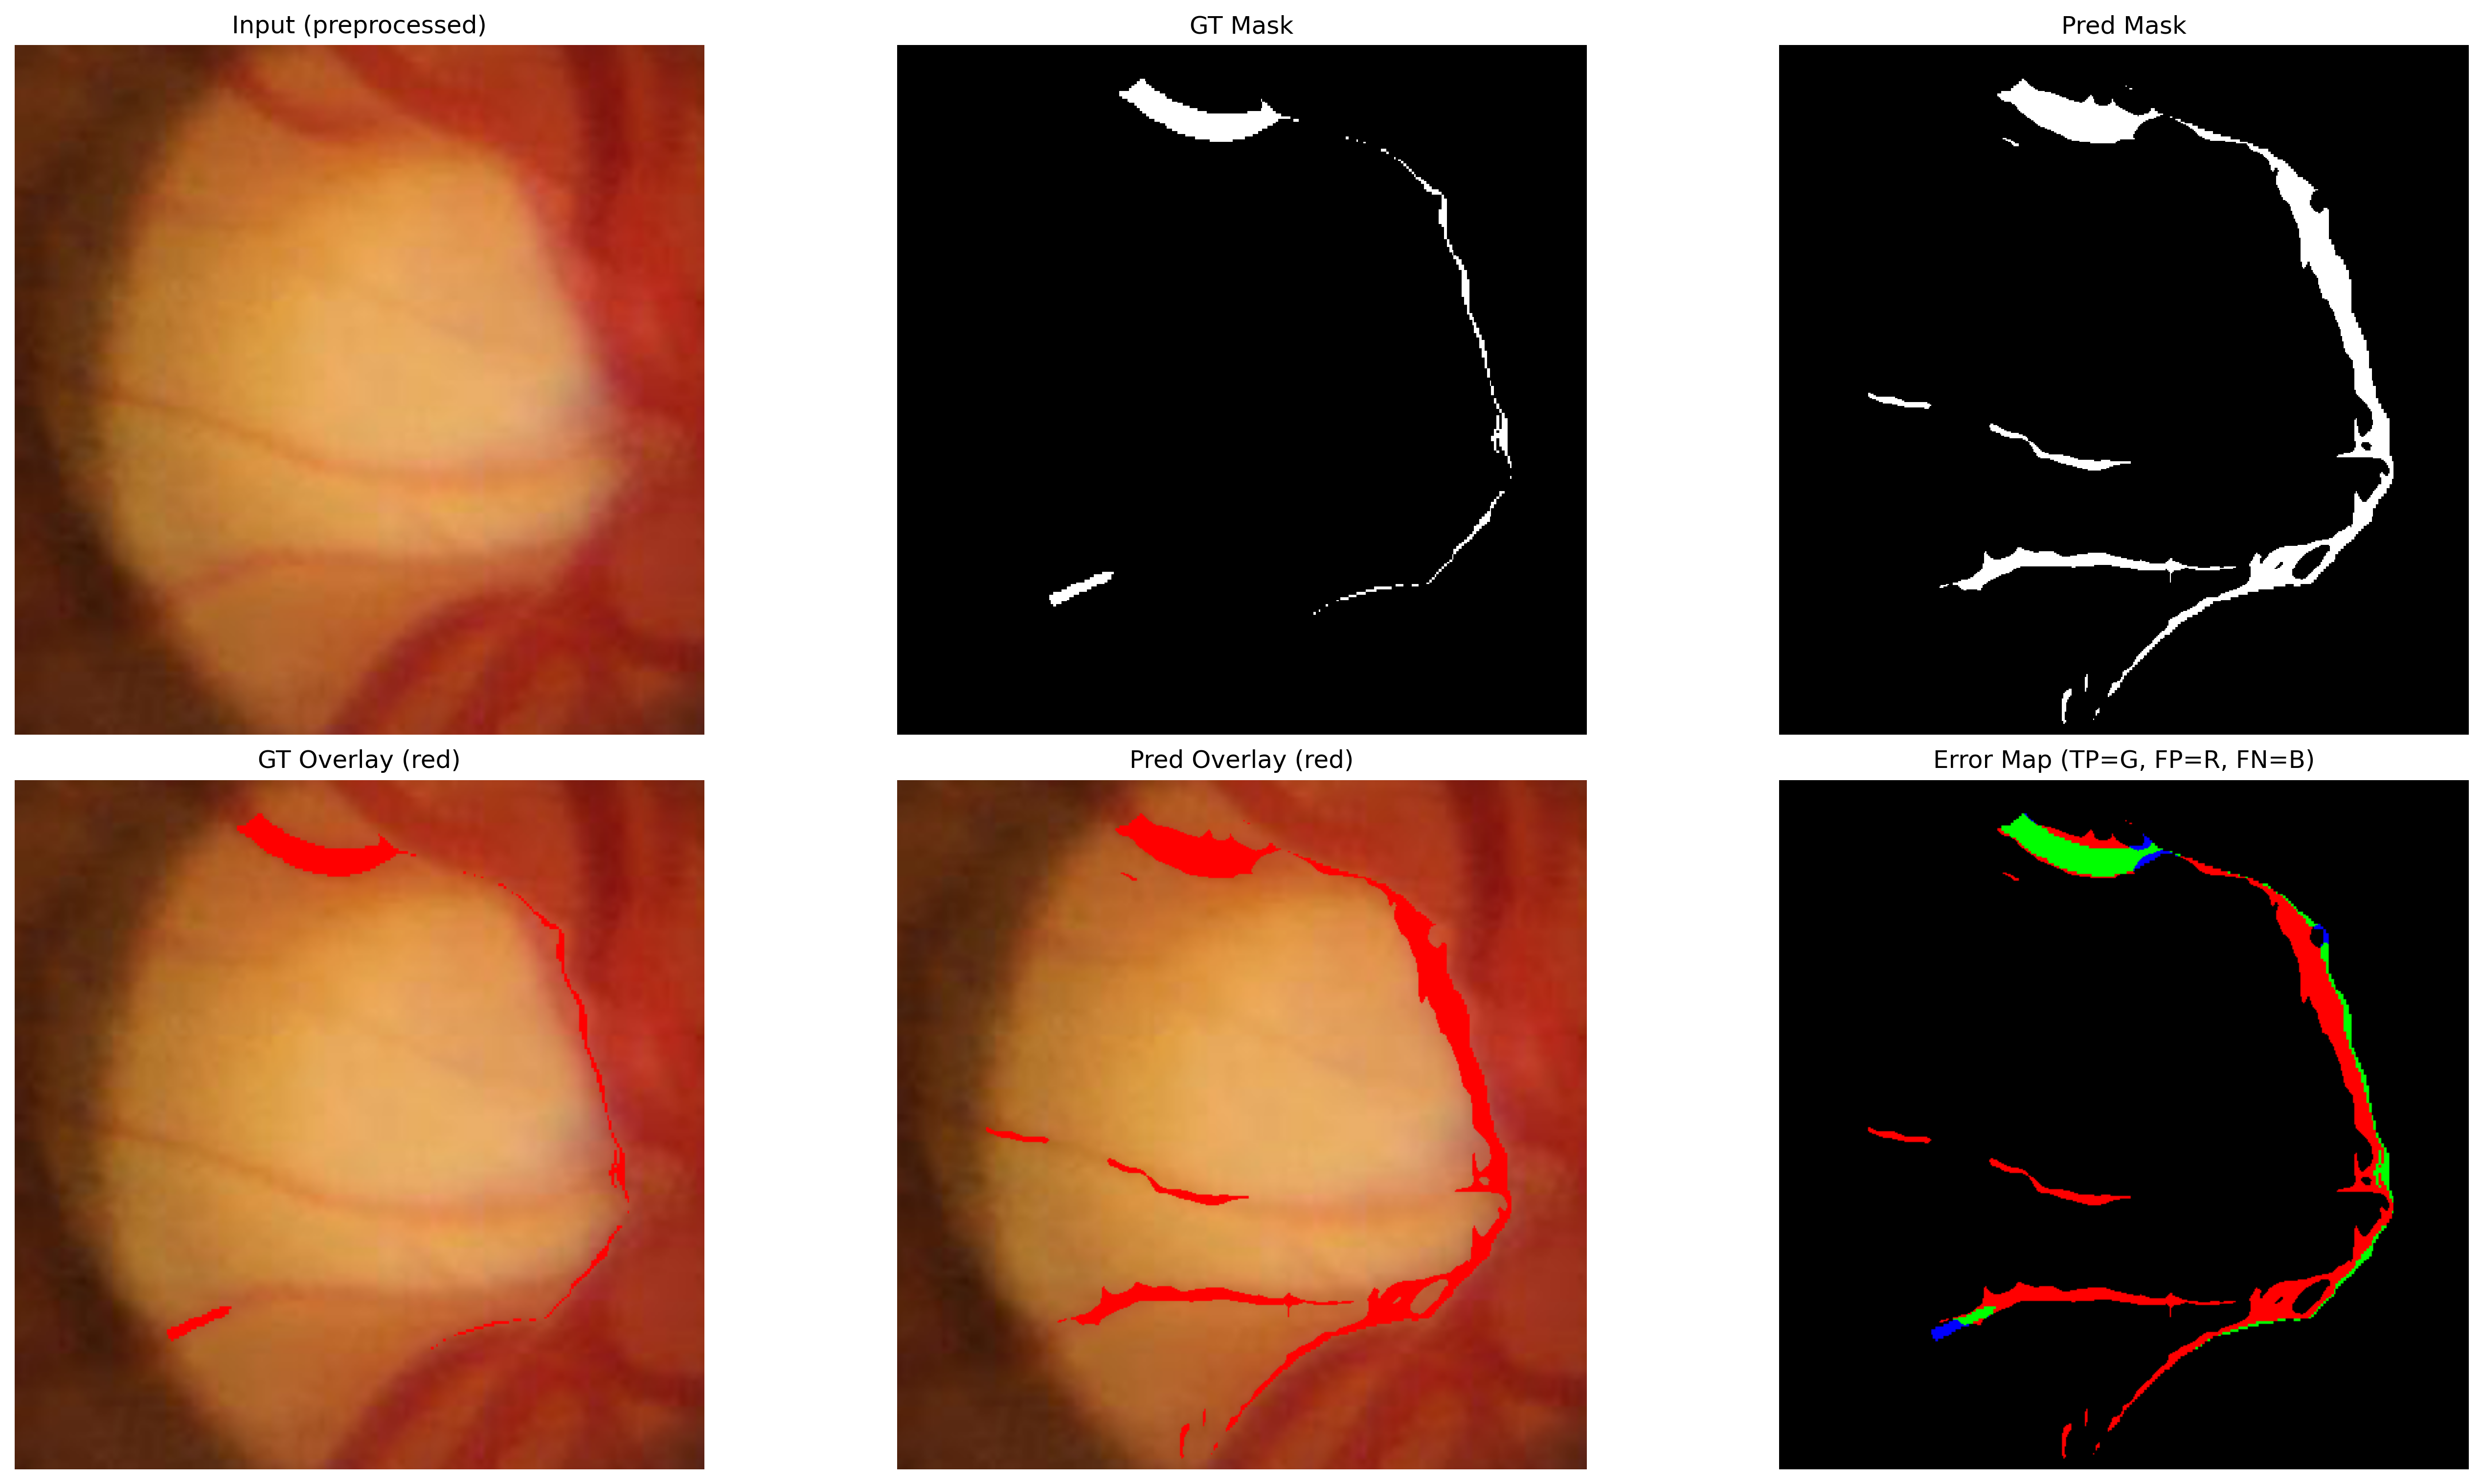
\includegraphics[width=0.48\linewidth]{figures/test_vis_112_G.png}\hfill
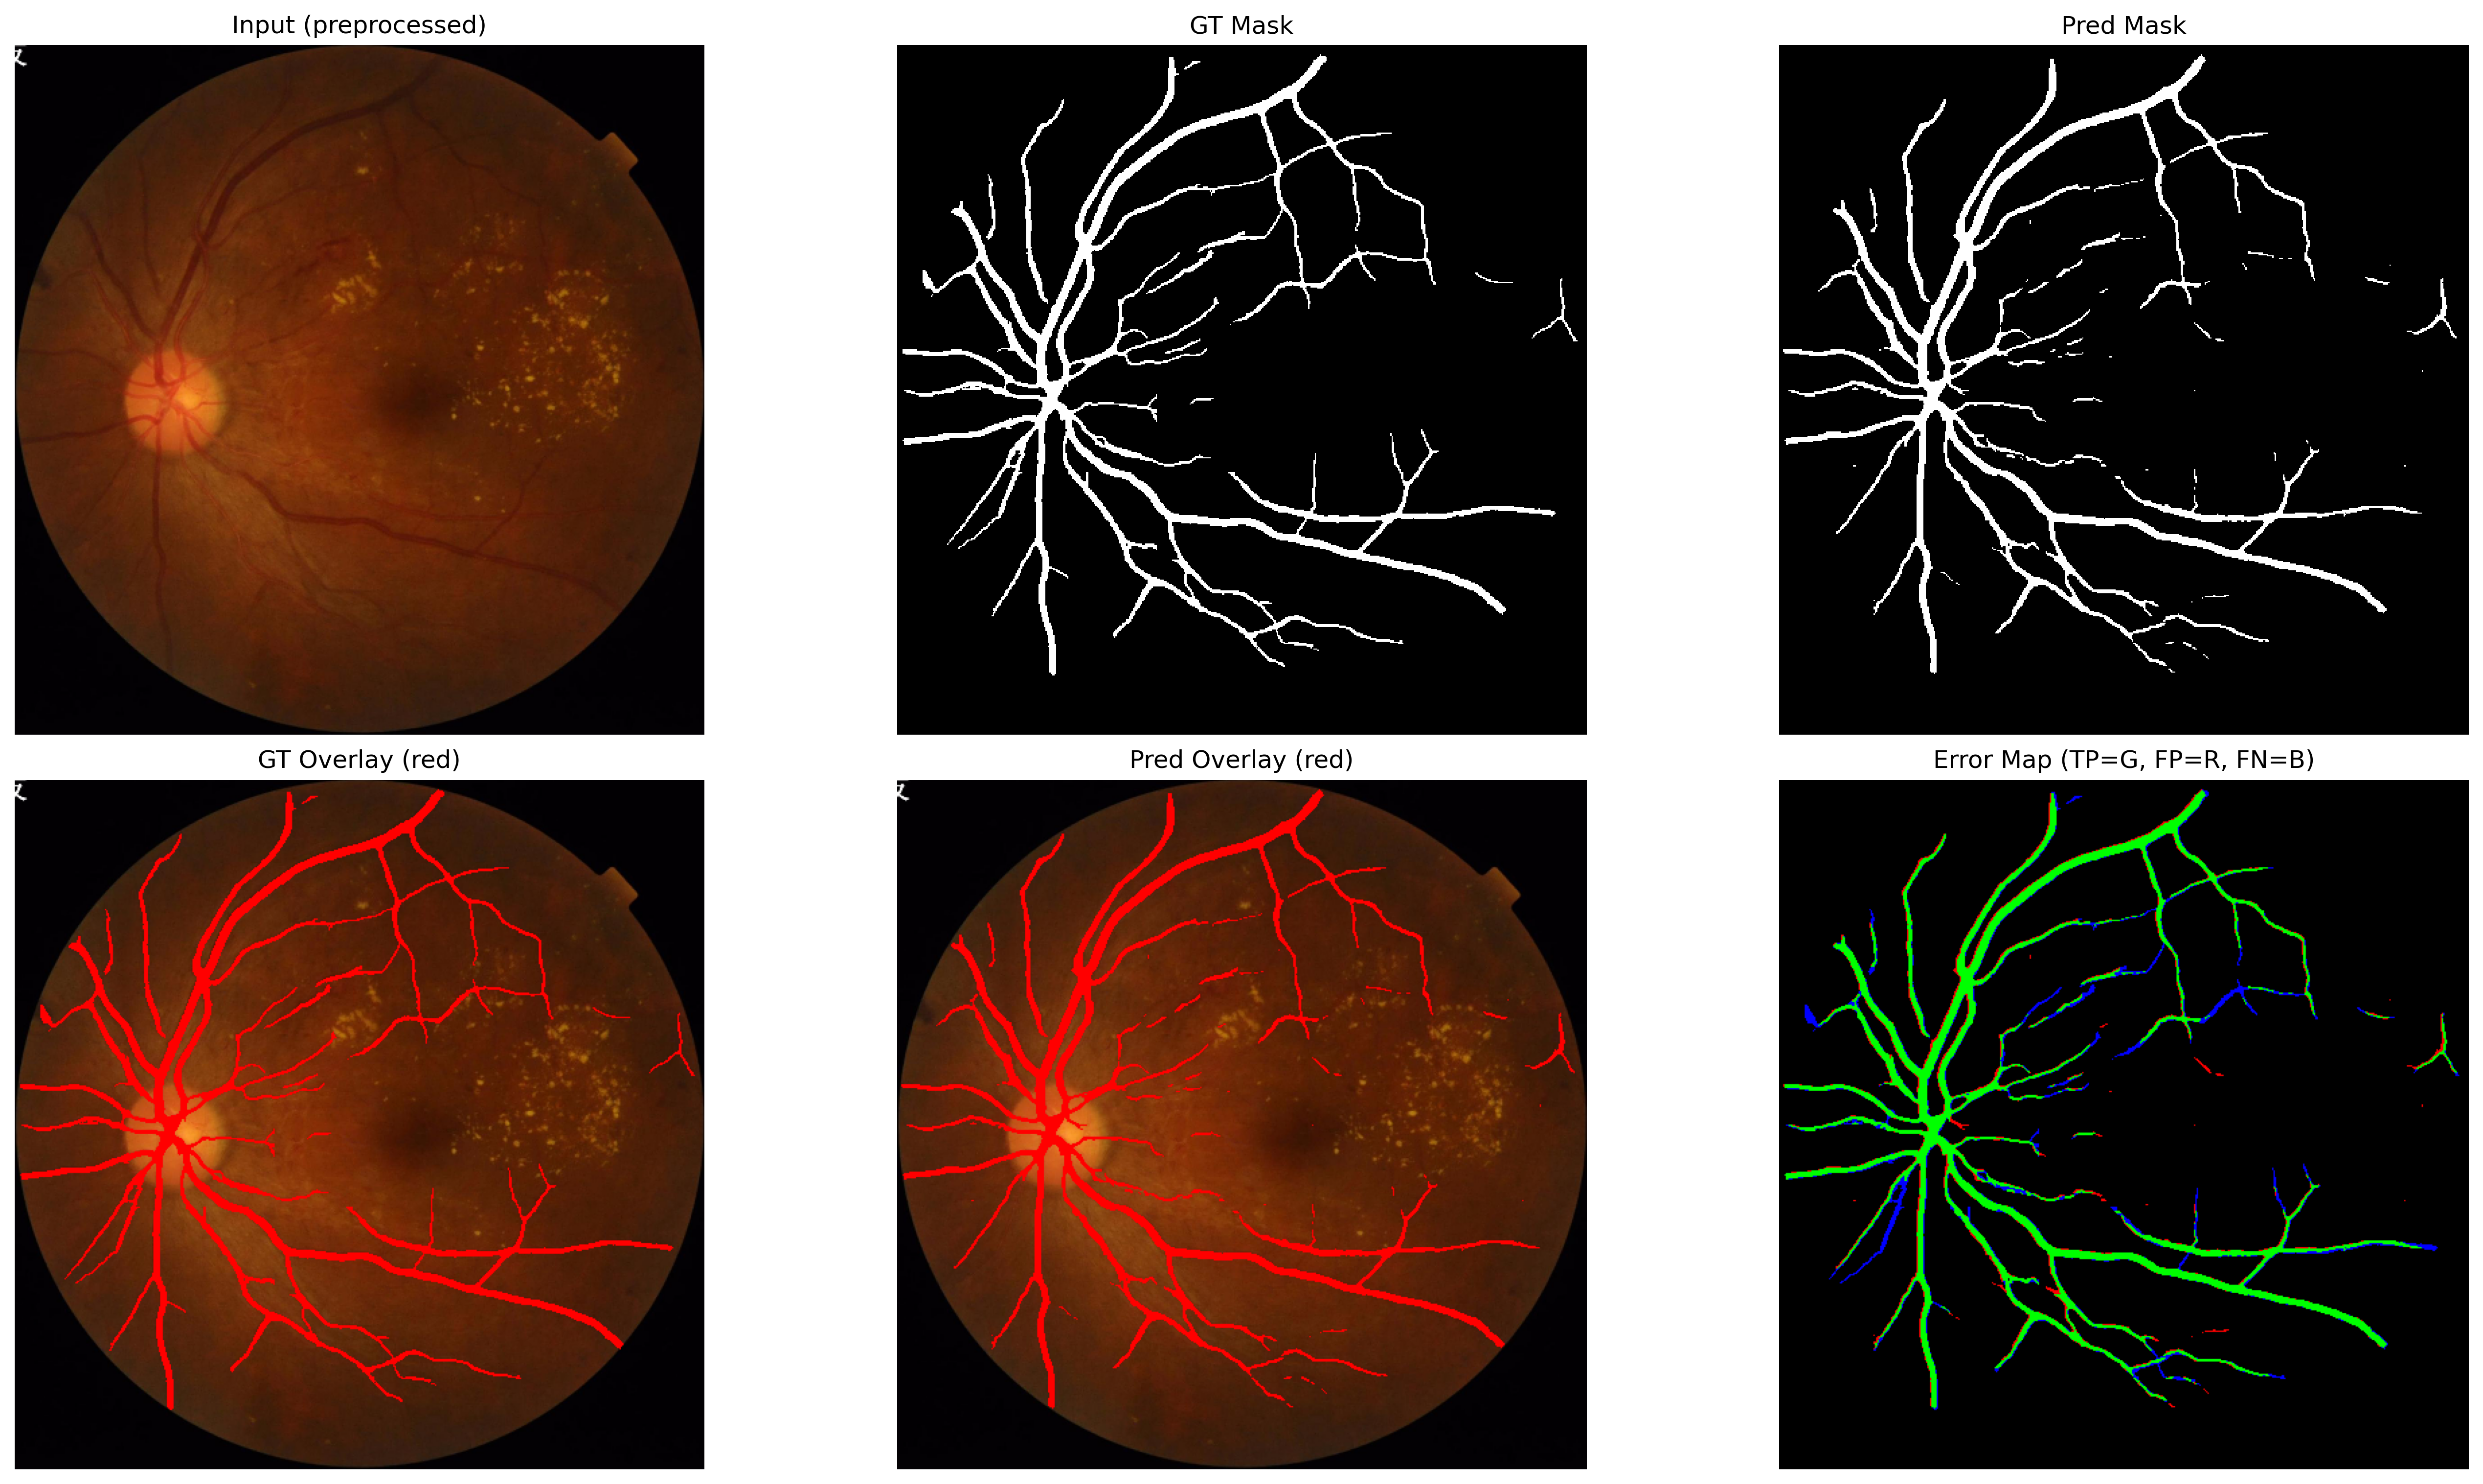
\includegraphics[width=0.48\linewidth]{figures/test_vis_90_D.png}
\caption{Seçili nitel örnekler: GT--tahmin karşılaştırmaları ve hata örüntüleri.}
\label{fig:qualitative}
\end{figure}

\subsection{Segmentasyon Sonrası Damar Analizi}
Segmentasyon çıktıları, damar yoğunluğu, iskelet uzunluğu ve dallanma sayısı açısından değerlendirilmiştir. Tablo~\ref{tab:vessel_analysis} sonuçları, damar yoğunluğunun ortalamada korunmasına karşın iskelet uzunluğu ve dallanma sayısında azalma eğilimi olduğunu göstermektedir.

\begin{table}[H]
\centering
\small
\caption{Damar analizi sonuçları (mean$\pm$std): GT ve model tahmini (Pred) karşılaştırması.}
\label{tab:vessel_analysis}
\begin{tabular}{lccc}
\toprule
\textbf{Gösterge} & \textbf{GT} & \textbf{Pred} & \textbf{Fark (Pred$-$GT)} \\
\midrule
Vessel density & $0.102824\pm0.039192$ & $0.103730\pm0.041278$ & $+0.000906\pm0.009618$ \\
Skeleton length (px) & $4830.675\pm1923.360$ & $4492.415\pm1730.630$ & $-338.260\pm452.431$ \\
Branch count & $277.445\pm139.570$ & $229.145\pm123.616$ & $-48.300\pm81.997$ \\
\bottomrule
\end{tabular}
\end{table}

\section{Tartışma}
Nicel sonuçlar, modelin test kümesinde dengeli bir precision/recall profili sergilediğini göstermektedir (Tablo~\ref{tab:test_macro}). Bununla birlikte, micro metriklerin macro metriklerden kısmen yüksek olması (Tablo~\ref{tab:test_micro}), daha yoğun damar içeren veya daha büyük alan kaplayan görüntülerin toplam piksel hesabında daha baskın olabildiğine işaret eder. Bu nedenle iki raporlama biçimi birbirini tamamlayıcı olarak değerlendirilmelidir.

Nitel örneklerde, hataların önemli bir kısmının ince damar uçlarında ve düşük kontrast bölgelerde yoğunlaştığı gözlenmiştir (Şekil~\ref{fig:qualitative}). Bu durum, segmentasyon metrikleri kabul edilebilir seviyede olsa dahi, damar topolojisinin tam korunmasını zorlaştırabilir. Nitekim damar analizi sonuçları, damar yoğunluğunun ortalamada benzer kaldığını, ancak iskelet uzunluğu ve dallanma sayısında azalma eğilimi olduğunu göstermektedir (Tablo~\ref{tab:vessel_analysis}). Bu tablo, özellikle ince damarların kopması veya süreksizleşmesi durumunda topolojik ölçümlerin daha duyarlı bir gösterge olabileceğini ortaya koyar.

Öte yandan, test kümesinde iki örnekte TP=FP=FN=0 durumu gözlenmiştir. Bu gibi “tam boş maske” örneklerinde metrikler tanım gereği 1.0 olarak hesaplanabilmektedir. Bu durum veri seti etiketleme içeriği veya ilgili örneklerde damar anotasyonunun bulunmaması gibi nedenlerle ortaya çıkabilir; raporlamada bu özel durum açıkça belirtilmelidir.

Bu çalışmanın başlıca sınırlılıkları; tek bir mimari (U-Net) ile sınırlı kalınması, sabit eşikleme stratejisinin (0.5) tüm görüntüler için optimal olmayabilmesi, ayrıca çıkarılan morfolojik göstergelerin daha ileri post-process (ör. küçük bileşen temizleme, skeleton pruning) adımları ile iyileştirilebilecek olmasıdır. Buna rağmen çalışma, FOV tabanlı ön işleme ve segmentasyon sonrası analiz ile uçtan uca tekrarlanabilir bir damar analizi hattı sunmaktadır.

\section{Sonuç ve Gelecek Çalışmalar}
Bu raporda, fundus retina görüntülerinde damar segmentasyonu ve segmentasyon çıktısından morfolojik damar göstergelerinin çıkarımı ele alınmıştır. FOV maskeleme tabanlı ön işleme ile retina dışı alanların etkisi azaltılmış; U-Net tabanlı model BCE ve Dice kaybı kombinasyonu ile eğitilmiştir. Test kümesinde macro ortalama Dice $0.8059\pm0.0752$ ve IoU $0.6807\pm0.0946$ elde edilmiştir. Segmentasyon sonrası analiz, damar yoğunluğunun ortalamada korunabildiğini; ancak iskelet uzunluğu ve dallanma sayısı gibi topolojik göstergelerde azalma eğilimi olabileceğini göstermiştir.

Gelecek çalışmalar kapsamında aşağıdaki iyileştirmeler planlanabilir:
\begin{itemize}
    \item Daha güçlü mimariler (ör. attention tabanlı U-Net varyantları) ile ince damarların daha iyi yakalanması,
    \item Kayıp fonksiyonu ve eşikleme stratejilerinin (ör. adaptif eşik, farklı loss kombinasyonları) sistematik biçimde araştırılması,
    \item Segmentasyon sonrası post-process adımları ile topolojik bütünlüğün artırılması ve morfolojik ölçümlerin daha kararlı hâle getirilmesi.
\end{itemize}


\printbibliography
\end{document}
